\documentclass{article}

\usepackage{hyperref}
\usepackage[T1]{fontenc}
\usepackage{graphicx}
\usepackage[utf8]{inputenc}


\title{%
Laboratorium 3\\
  \huge Interpolacja}
\author{Mateusz Król}
\date{12/03/2024 r.}

\begin{document}
\maketitle


\section*{Zadanie 1.}
\textbf{Populacja Stanów Zjednoczonych na przestrzeni lat przedstawiała
się następująco:}
\begin{center}
  \begin{tabular}{c c} 
   Rok & Populacja\\
   1900 & 76 212 168\\
   1910 & 92 228 496\\
   1920 & 106 021 537\\
   1930 & 123 202 624\\
   1940 & 132 164 569\\
   1950 & 151 325 798\\
   1960 & 179 323 175\\
   1970 & 203 302 031\\
   1980 &226 542 199
  \end{tabular}
\end{center}
\textbf{Istnieje dokładnie jeden wielomian ósmego stopnia, który interpoluje
 powyższe dziewięć punktów, natomiast sam wielomian może być reprezentowany na różne sposoby.}
\\\\
Przykładowe dane:
\begin{figure}[ht!]
  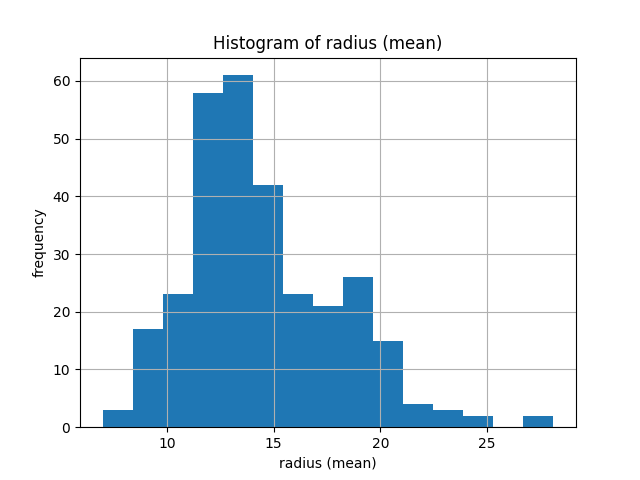
\includegraphics[width=\linewidth]{figures/hist.png}
\end{figure}
\begin{figure}[ht!]
  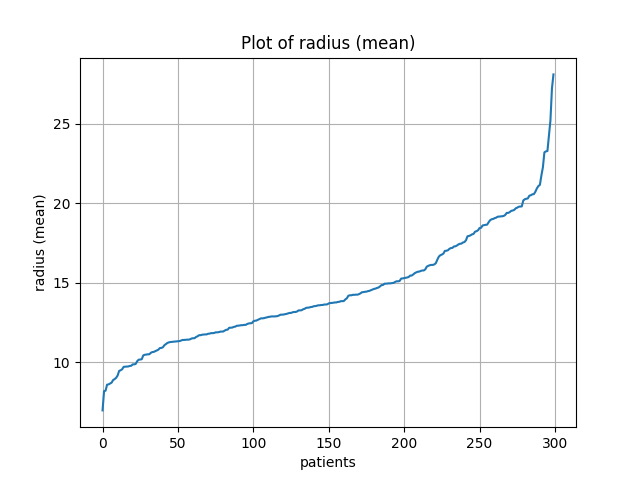
\includegraphics[width=\linewidth]{figures/plot.png}
\end{figure}
\\
Korzystając z $A_{lin}$ - liniowej reprezentacji oraz $A_{quad}$ - 
kwadratowej reprezentacji danych z pierwszego zbioru dostarczonego do zadania, jesteśmy w 
stanie wyznaczyć wektor wag $w$:
$$ A^T \cdot A \cdot w = A^T \cdot b$$
W tym celu wykorzystuję funkcję \textit{scipy.linalg.solve}, służącą do rozwiązywania 
układów równań liniowych, z biblioteki \textit{SciPy}. \\\\
Współczynniki uwarunkowania macierzy liczę korzystając z funkcji \textit{numpy.linalg.cond} 
z biblioteki \textit{NumPy}.
Wartości wyniosły:
\begin{itemize}
  \item dla reprezentacji liniowej - $cond(A^T\cdot A)\approx 1.81\cdot 10^{12}$
  \item dla reprezentacji kwadratowej - $cond(A^T\cdot A)\approx 9.06\cdot 10^{17}$
\end{itemize}
Następnie wyznaczając wektor $p$ na podstawie danych z drugiego zbioru dostarczonego do
zadania i porównując go z wartościami prawdziwymi, jesteśmy w stanie oszacować dokładność
metody dla różnych reprezentacji macierzowych danych:
\begin{center}
  \begin{tabular}{  |c|c|c| } 
   \hline
   Matrix representation & false-positives & false-negatives\\
   \hline
   linear & 6 & 2\\
   \hline
   quadratic & 15 & 5\\
   \hline
  \end{tabular}
\end{center}
\subsection*{Wnioski}
\null\quad Reprezentacja liniowa okazała się być dokładniejsza dla dostarczonych
zbiorów danych - zapewniła mniejszy współczynnik uwarunkowania oraz zwróciła mniejszą
ilość wyników fałszywych niż reprezentacja kwadratowa.


\end{document}